\documentclass{article}
\usepackage[utf8]{inputenc}
\usepackage{graphicx, amsmath}

\title{Salient Features of Cosmology - PHY 563}
\author{Lia Hankla}
\date{Due 21 February 2017}

\begin{document}

\maketitle
The ``Comments'' page evaluates the current evidence and some experimental techniques for measuring relevant quantities. The second page, ``Evidence'', ranks references from most solid/recent at the top of the page to least solid at the bottom.

\newpage
\section{Homogeneity \& Isotropy: Comments}
On the whole the CMB seems pretty isotropic. However, there are unexplained fluctuations with amplitudes on the order of $10^{-5}$ that make me hesitant, as noted in Ref 1 and 2. Ref. 3 explicitly calculates how big homogeneities could be and still go undetected in the CMB, which I thought was an interesting idea. 

\newpage
\section*{Homogeneity \& Isotropy: Evidence}

\subsection*{1. Schwarz et al 2016: CMB Anomalies after Planck}
\begin{itemize}
\item Unexplained anomalies: hemispherical asymmetry, cold spot, etc.
\item Where do quadrupole and octopole come from?
\end{itemize}

\subsection*{2. Zibin and Moss 2014: Nowhere to hide: Closing in on Cosmological Homogeneity}
\begin{itemize}
\item Use various CMB anomalies to constrain homogeneity (gravitational lensing, other effects)
\item Calculate largest structures that would not be detected in secondary CMB spectrum (figure)
\end{itemize}

\begin{figure}[h]
\begin{center}
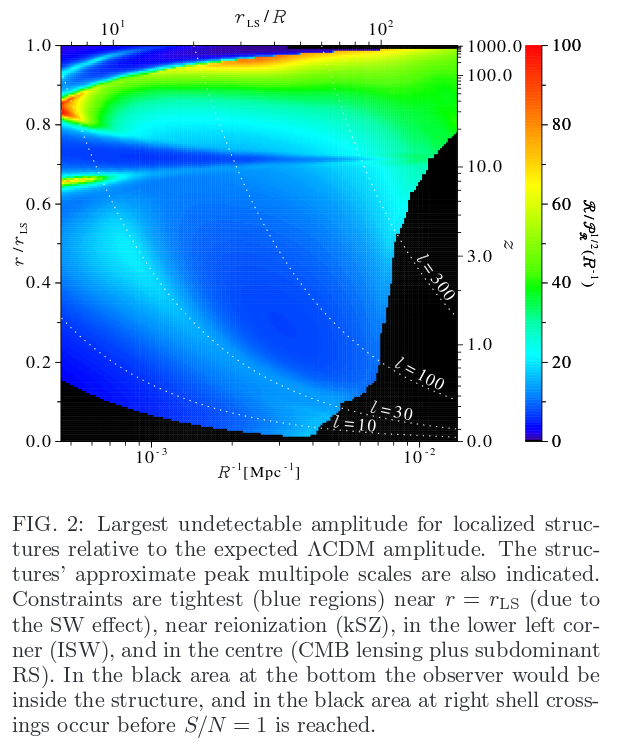
\includegraphics[width=.7\textwidth,angle=0.]{homogeneity.png}
\end{center}
\caption{Scale of structures that wouldn't be detectable in CMB secondary spectrum. From Ref. 3}
\end{figure}



\newpage
\section{Uniform Expansion: Comments}
Progress is still being made regularly on this front (especially measuring the Hubble constant). Lots of collaborations have entertaining names (H0LiCOW, for instance). The methods range from using the CMB, as in WMAP (Ref. 3 below) and independent measurements based off of quasar and Cepheid variable distance measurements (Ref. 1 and 2, respectively). While these are all quite recent, I ranked the quasar images higher in plausibility because they were independent from the CMB papers (which always just fit to the standard 6-parameter model) and agreed with the Cepheid variable estimates in Ref. 2. This study was also attractive since it avoided confirmation bias; however, the analysis itself was sensitive to knowing the mass distribution of the lensing quasar, which makes it a little dubious. 

 
\newpage
\section*{Uniform Expansion: Evidence}
\subsection*{1. Bonvin et al 2016: H0LiCOW}
\begin{itemize}
\item Quasar images, time-delay distances depend on matter distribution
\item Avoid confirmation bias (blind to cosmological parameters)
\item H0=71.9 km/sMpc.
\item A little sketchy because lens mass distribution could fit observed form but result in different time-delay difference.
\end{itemize}

\subsection*{2. Riess et al 2016: A 2.4\% Determination of the Local Value of the Hubble Constant}
\begin{itemize}
\item Uses HST to observe Cepheid variables
\item 2.4\% uncertainty, conflicts with LCDM prediction (tension!)
\end{itemize}

\begin{figure}[h]
\begin{minipage}[b]{.6\textwidth}
\begin{center}
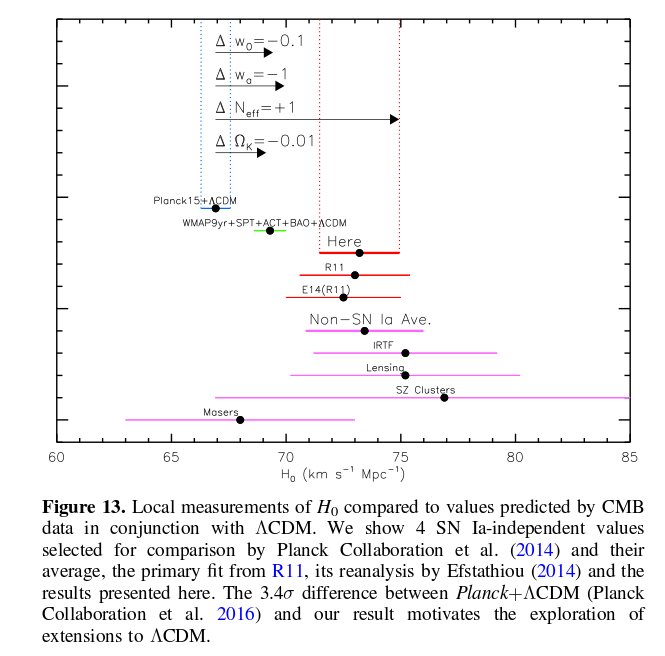
\includegraphics[width=\textwidth,angle=0.]{hubble1.png}
\end{center}
\caption{Comparison of measurements of Hubble Constant. From Ref. 2}
\end{minipage}
\hfill
\begin{minipage}[b]{.4\textwidth}
\begin{center}
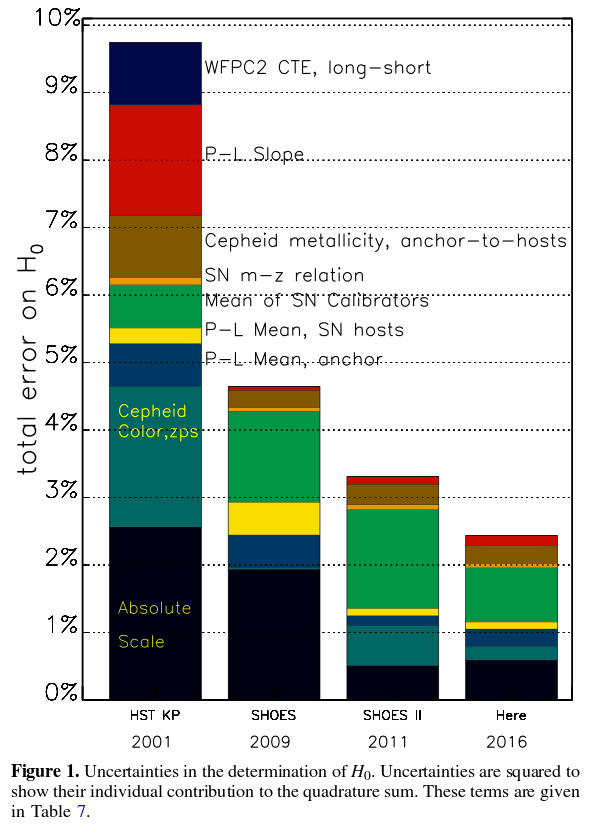
\includegraphics[width=\textwidth,angle=0.]{hubble2.png}
\end{center}
\caption{Comparison of error in measuremets of Hubble constant. From Ref. 2}
\end{minipage}
\end{figure}

\subsection*{3. Hinshaw et al 2013: Nine-Year WMAP Observations}
\begin{itemize}
\item Determine Hubble constant to 1.5\% precision.
\item Fit to 6-parameter LCDM model
\end{itemize}


\newpage
\section{Spatially Flat: Comments}
There seems to be pretty good evidence for the flatness of the universe, although everything I found calculated $\Omega_K$ by subtracting all the other densities added up from 1, i.e. $\Omega_K=1-\Omega_{\mathrm{tot}}$. It would be interesting to find other methods of measuring the flatness. Maybe somebody has measured the angles of an extremely large triangle somewhere, but I didn't come across such an experiment. 

\newpage

\section*{Spatially Flat: Evidence}

\subsection*{1. Planck Collaboration 2016: Planck 2015 Results}
\begin{itemize}
\item Hubble constant H0=$67.8\pm.9$ km/s/Mpc
\item $|\Omega_K|<.005$
\item Fit to 6-parameter model
\end{itemize}

\begin{figure}[h]
\begin{center}
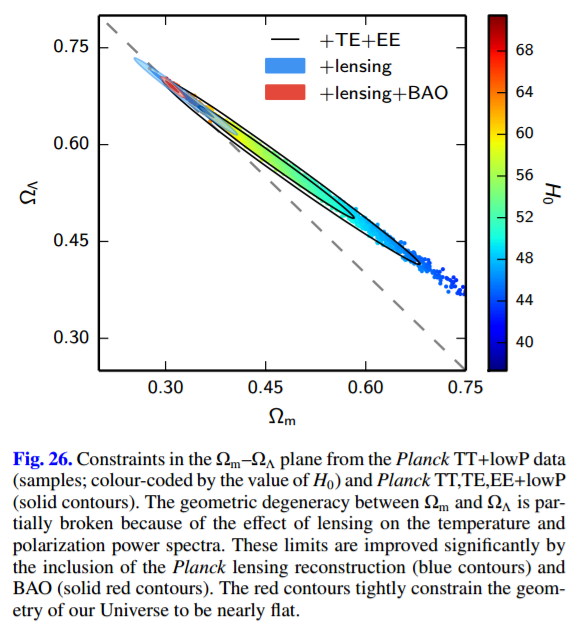
\includegraphics[width=.8\textwidth,angle=0.]{spatialFlatness.png}
\end{center}
\caption{Constraints on the flatness of the universe. From Ref. 1}
\end{figure}

\subsection*{2. Hinshaw et al 2013: Nine-year WMAP Observations, Cosmological Parameter Results}
\begin{itemize}
\item Spatial curvature parameter $\Omega_k=-.0027^{+.0039}_{-.0038}$
\item Fit to 6-parameter model
\end{itemize}

\newpage
\section{Thermal Background Radiation: Comments}
Evidence that the CMB is at 2.7 K seems pretty solid. It has been measured multiple times and Ref. 1 has compiled many different accounts and takes instrumental variation into consideration. Its relatively recent discovery and the fact that we see galaxies and stars in front of this radiation seems like pretty good evidence to me that the CMB is indeed background radiation. 

\newpage
\section*{Thermal Background Radiation: Evidence}
\subsection*{1. Fixsen 2009: The Temperature of the CMB}
\begin{itemize}
\item Independent from WMAP
\item Accounts for experimental calibration and error
\item CMB temperature =2.7260K$\pm1.3$mK
\end{itemize}

\begin{figure}[h]
\begin{center}
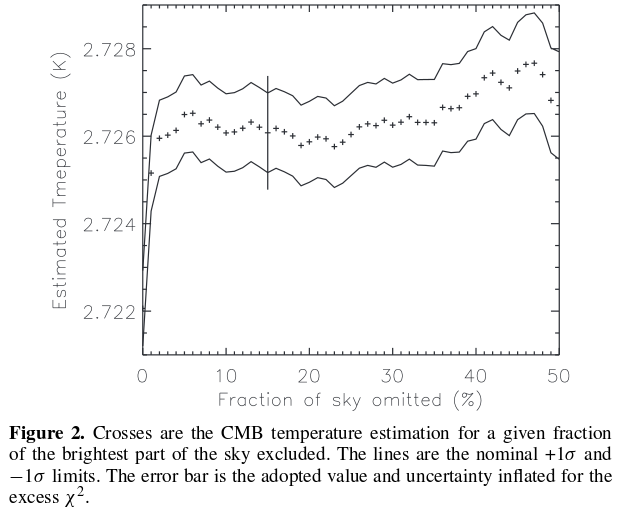
\includegraphics[width=.8\textwidth,angle=0.]{cmbTemp.png}
\end{center}
\caption{Temperature of the CMB. From Ref. 1}
\end{figure}


\newpage
\section{Chemical Composition: Comments}
It seems like the chemical composition of the universe is pretty well established and has been for a while (1970s). There is still ongoing debate about the early universe's composition, especially relating to star formation, but we can observe today's distribution from looking at the sun and meteors. I ranked two sources; Ref. 1 is more current but gets most of its data from Ref. 2. 

\newpage
\section*{Chemical Composition: Evidence}
\subsection*{1. N. N. Greenwood, A. Earnshaw 2012: Chemistry of the Elements}

\begin{figure}[h]
\begin{center}
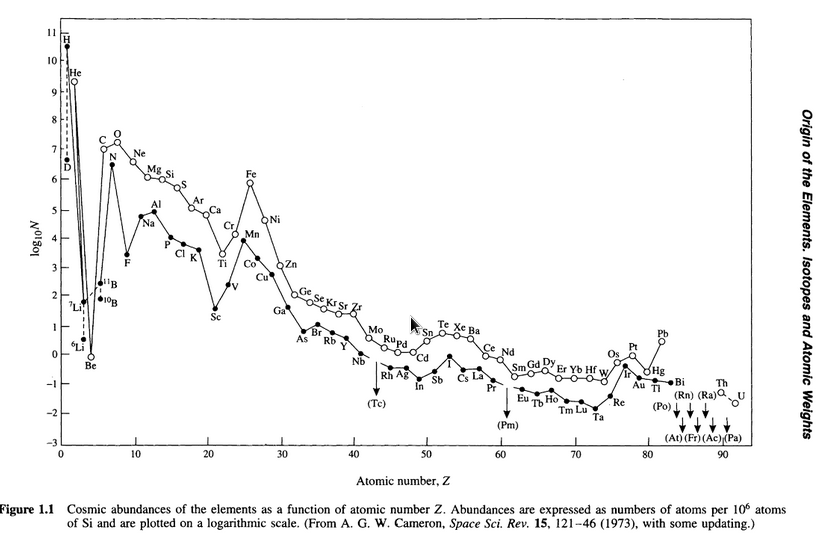
\includegraphics[width=.8\textwidth,angle=0.]{abundances.png}
\end{center}
\caption{Abundances of elements in the solar system. From Ref. 1}
\end{figure}

\subsection*{2. Cameron 1973: Abundances of the elements in the solar system}
\begin{itemize}
\item Spectroscopic evidence (solar, cosmic ray), meteor samples
\item 74\% hydrogen, 24\% helium, 2\% trace
\end{itemize}


\newpage
\section{Matter-Antimatter Imbalance: Comments}
Overall, the evidence for this feature is pretty solid. Recent 2016 balloon experiments (Ref. 1 on next page) have pushed the upper limit on the antihelium-helium ratio even lower, to a 95\% confidence level. Previous papers from the 1980s and 1990s have also established that no large-scale antimatter pockets exist in the observable universe (although small pockets are not ruled out). These use CMB flux (Ref. 2) and big-bang theory and $\gamma$-astronomy (Ref. 3) to predict the abundance of antimatter. A sketchier method appeared more recently in 2003, using the annihilation spectrum from anti-meteorites coming into contact with matter to predict abundances (Ref. 4). This piece of evidence is ranked lower due to its dependence on only one number (the average number of asteroids that hit earth).

\newpage
\section*{Matter-Antimatter Imbalance: Evidence}
\subsection*{1. Abe et al 2016: The results from BESS-Polar experiment}
\begin{itemize}
\item Balloon experiments measure spectrum of cosmic-ray antiprotons
\item Their Fig. 8 = antihelium/helium limits and comparison to other limits, $7e10^{-8}$ at 95\% confidence upper limit. Reproduced below.
\item LOWEST upper bound yet.
\end{itemize}

\begin{figure}[h]
\begin{center}
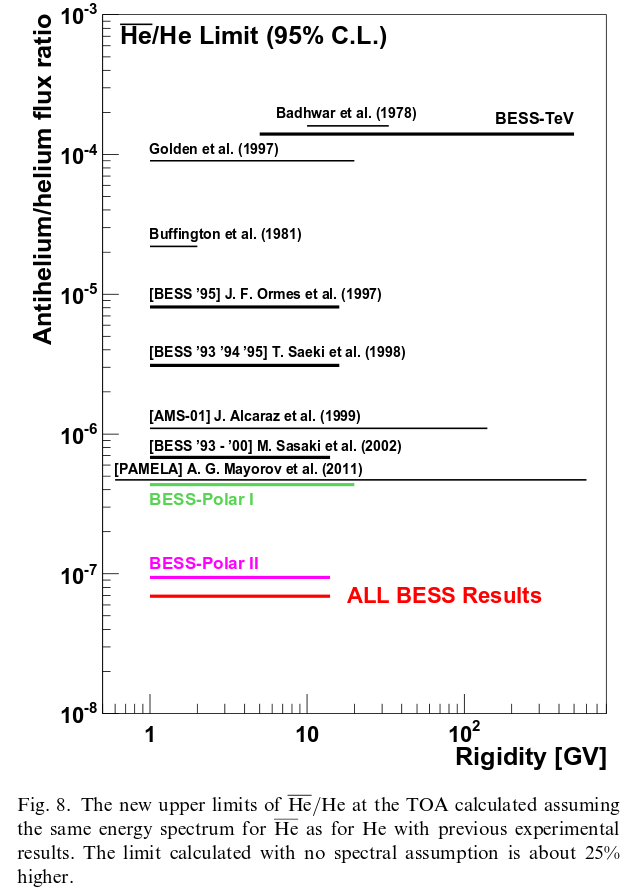
\includegraphics[width=.4\textwidth,angle=0.]{antimatter.png}
\end{center}
\caption{Antimatter-matter asymmetry bounds. From Ref. 1}
\end{figure}

\subsection*{2. Cohen, De Rujula, Glashow 1997: A Matter-Antimatter Universe?}
\begin{itemize}
\item Matter-antimatter annihilation would lead to a $\gamma$-ray background and distort the CMB...using CMB measurements can get limit on ratio. (Lower bound on CMB signal due to annihilation rate...find that CMB flux would be several orders of magnitude higher than what was seen experimentally by COMPTEL (Fig. 5), even to within error bars.
\item shows no LARGE-SCALE, doesn't rule out small pockets
\end{itemize}

\subsection*{3. Chechetkin, Khlopov, Sapozhnikov 1982: Astrophysical Aspects of antiproton interaction...}
\begin{itemize}
\item Use big-bang cosmology to predict abundances of antiprotons, then would influence light elements distribution. Ratio of antimatter to matter: theory and experiment. Creation of antibaryons from primordial black holes--get from cosmological density. 
\item $\gamma$-astronomy.
\end{itemize}


\subsection*{4. Fargion and Khlopov 2003: Antimatter bounds from antiasteroid annihilation...}
\begin{itemize}
\item Bound from absence of anti-meteorite annihilation: $10^{-9}$.
\item Dubious: depends on estimates of present flux of meteorites on Earth, signal can't be detected by Batse (so $r\le 10^{-9}$).
\end{itemize}

\newpage
\section{Singularity: Comments}
Overall the evidence for this feature is mostly indirect, i.e. mostly models that extrapolate to times that we can see and purport to explain that. Interestingly, when I searched Google Scholar for ``cosmology singularity'', most results that appeared were alternatives to a singularity or constraints on future singularities. Ref. 1, for instance, suggests how to use low redshift observations to rule out or support bouncing models. Ref. 2 is older and also mostly theoretical. It does, however, suggest that observational evidence could support a non-singular model. As a result I am not very convinced on this point. 

\newpage
\section*{Singularity: Evidence}
\subsection*{1. Cai et al 2016: Searching for a matter bounce cosmology with low redshift observations}
\begin{itemize}
\item Low redshift observations can pass judgment on bouncing cosmologies
\end{itemize}

\subsection*{2. Ellis and Maartens 2003: The emergent universe: inflationary cosmology with no singularity}
\begin{itemize}
\item Not observationally-based except to note that $\Omega_K$ could potentially be positive, and that we should consider a closed universe that would also inflate.
\end{itemize}

\newpage
\section{Scale-Invariant Fluctuations: Comments}
Although the limit of tensor-to-scalar ratio has a decently tight upper limit (Ref 1 and 2), non-Gaussianity can explain some of the unresolved anisotropies in the CMB spectrum (Ref 3). I am hence not very convinced on this front. 

\newpage
\section*{Scale-Invariant Fluctuations: Evidence}
\subsection*{1. Planck Collaboration 2016: Planck 2015 Results}
\begin{itemize}
\item Upper limit on tensor-to-scalar ratio: $r<.09$
\end{itemize}

\subsection*{2. Hinshaw et al 2013: Nine-year WMAP Observation}
\begin{itemize}
\item Measure fluctuation amplitude to 3\% precision.
\item Limits on tensor fluctuation relative to density fluctuations: $r<0.13$
\end{itemize}

\subsection*{3. Adhikari et al 2016: Large-scale anomalies in the CMB as signatures of non-Gaussianity}
\begin{itemize}
\item Explain power spectrum asymmetry via non-Gaussian density fluctuations
\end{itemize}

\newpage
\section{Hierarchy of Structure: Comments}
I remember the figure on the next page of the power spectrum as being one of the most well-fit in cosmology. So it seems like the evidence for a characteristic length scale is pretty good. I only listed one reference, but all sorts of papers have the same graph (the Planck Collaboration results, for example). 


\newpage
\section*{Hierarchy of Structure: Evidence}
\subsection*{1. Hinshaw et al 2013: Nine-year WMAP Observations}
\begin{itemize}
\item Angular power spectrum shows clear peak at around $l\sim250$
\item Angular power spectrum amplitude measured to within 3\%
\end{itemize}

\begin{figure}[h]
\begin{center}
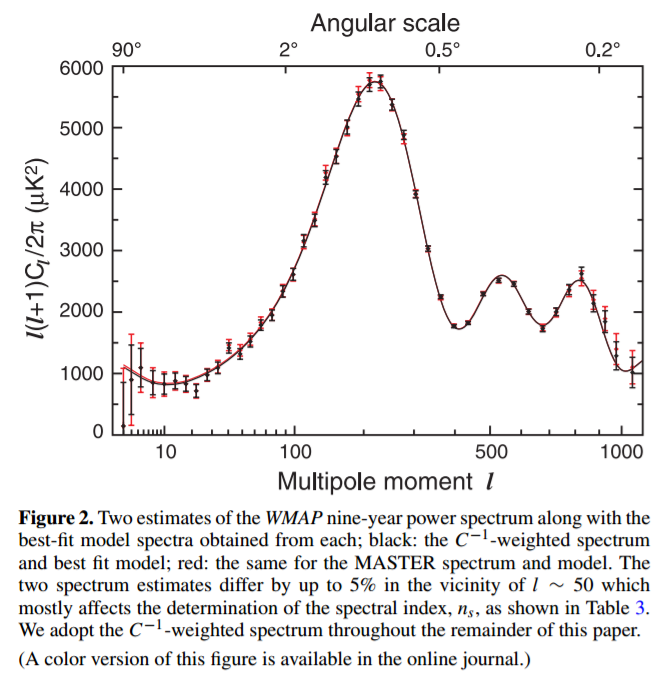
\includegraphics[width=\linewidth,angle=0.]{powerSpectrum.png}
\end{center}
\caption{Power spectrum showing the hierarchy of length scales. From Ref. 1}
\end{figure}

\newpage
\section{Ordinary Matter Mass Proportion: Comments}
Some papers I found fit to the standard 6-parameter cosmological model, which fits well but of course is just a parameterization, but still strong (Refs. 1 and 2). The other classic evidence for dark matter comes from rotation curves, which seem to deviate from what one would expect from estimates of the mass from observed stars and Newtonian physics. I rank the evidence from Ref. 3 last because there are alternate explanations for the rotation curve problem, such as modified newtonian dynamics. 

\newpage
\section*{Ordinary Matter Mass Proportion: Evidence}
\subsection*{1. Planck Collaboration 2016: Planck 2015 Results}
\begin{itemize}
\item $\Omega_b/(\Omega_b+\Omega_c)=.022/(.022+.12)\approx.155$
\item Best fit to 6-parameter model
\item See figure in the ``Mass Energy Proportion: Evidence'' section for constraints on $\Omega_b$ and $\Omega_c$.
\end{itemize}

\subsection*{2. Bennett et al 2003: First-year WMAP Observations}
\begin{itemize}
\item Fit to cosmological model: 4.4\% baryons, 22\% dark matter, 73\% dark energy.
\end{itemize}

\subsection*{3. Hashim et al 2014: Rotation Curve with MOND and Dark Matter Halo profile for ESO138-G014}
\begin{itemize}
\item Take data from many different sources (Cepheids, HII clouds, etc.) 
\item MOND would be opposite evidence for dark matter
\end{itemize}

\begin{figure}[h]
\begin{minipage}[b]{.5\textwidth}
\begin{center}
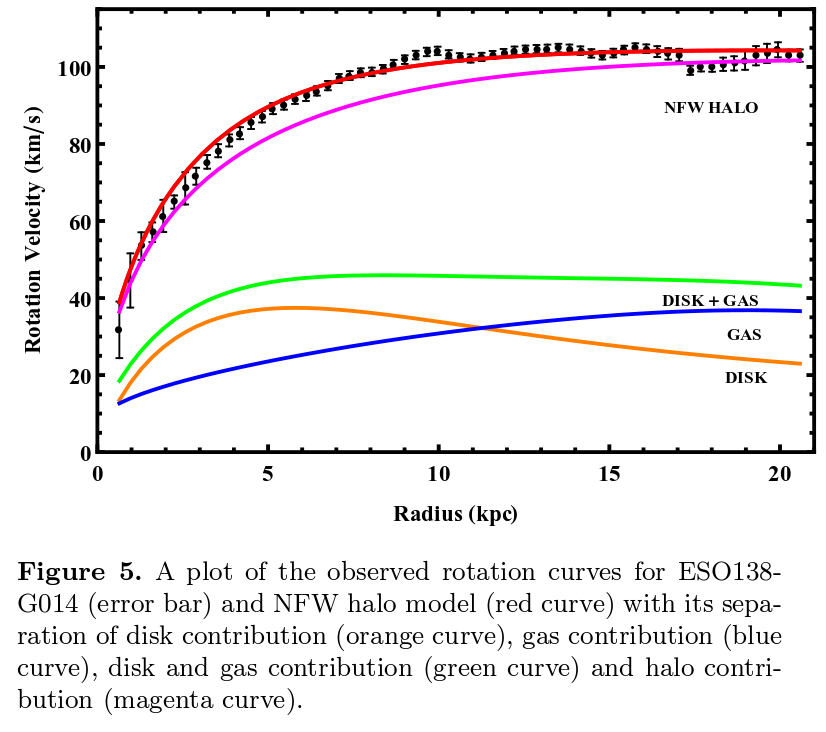
\includegraphics[width=\textwidth,angle=0.]{rcDarkMatter.png}
\end{center}
\caption{Dark matter halo prediction of rotation curve. From Ref. 3}
\end{minipage}
\hfill
\begin{minipage}[b]{.5\textwidth}
\begin{center}
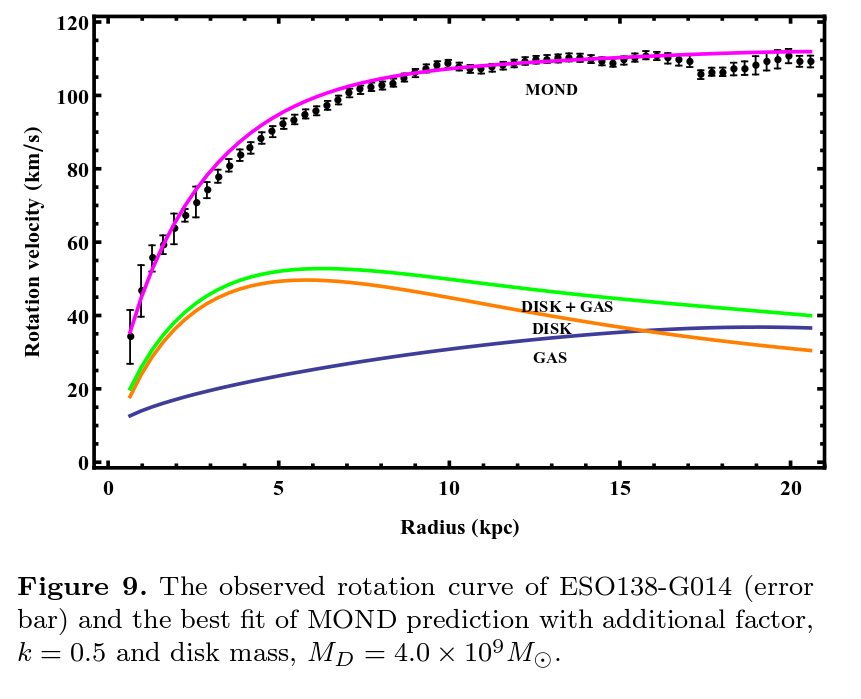
\includegraphics[width=\textwidth,angle=0.]{mond.png}
\end{center}
\caption{MOND prediction of rotation curve. From Ref. 3}
\end{minipage}
\end{figure}


\newpage
\section{Mass Energy Proportion: Comments}
Since there is an independent measurement given by supernovae measurements, the $\Lambda$CDM model is tested in a way. Unfortunately it seems to disagree with other methods in deciding what $\Omega_\Lambda$ is, which means that more (precise and independent) evidence is needed. The figure on the next page contains constraints for most of the $\Lambda$CDM variables and so applies to some other sections as well.

\newpage
\section*{Mass Energy Proportion: Evidence}
\subsection*{1. Planck Collaboration 2016: Planck 2015 Results}
\begin{itemize}
\item $\Omega_m=.315\pm0.017$, 
\item Conflicts with Type 1a supernovae measurements of $\Omega_m\approx0.23$
\end{itemize}

\begin{figure}[h]
\begin{center}
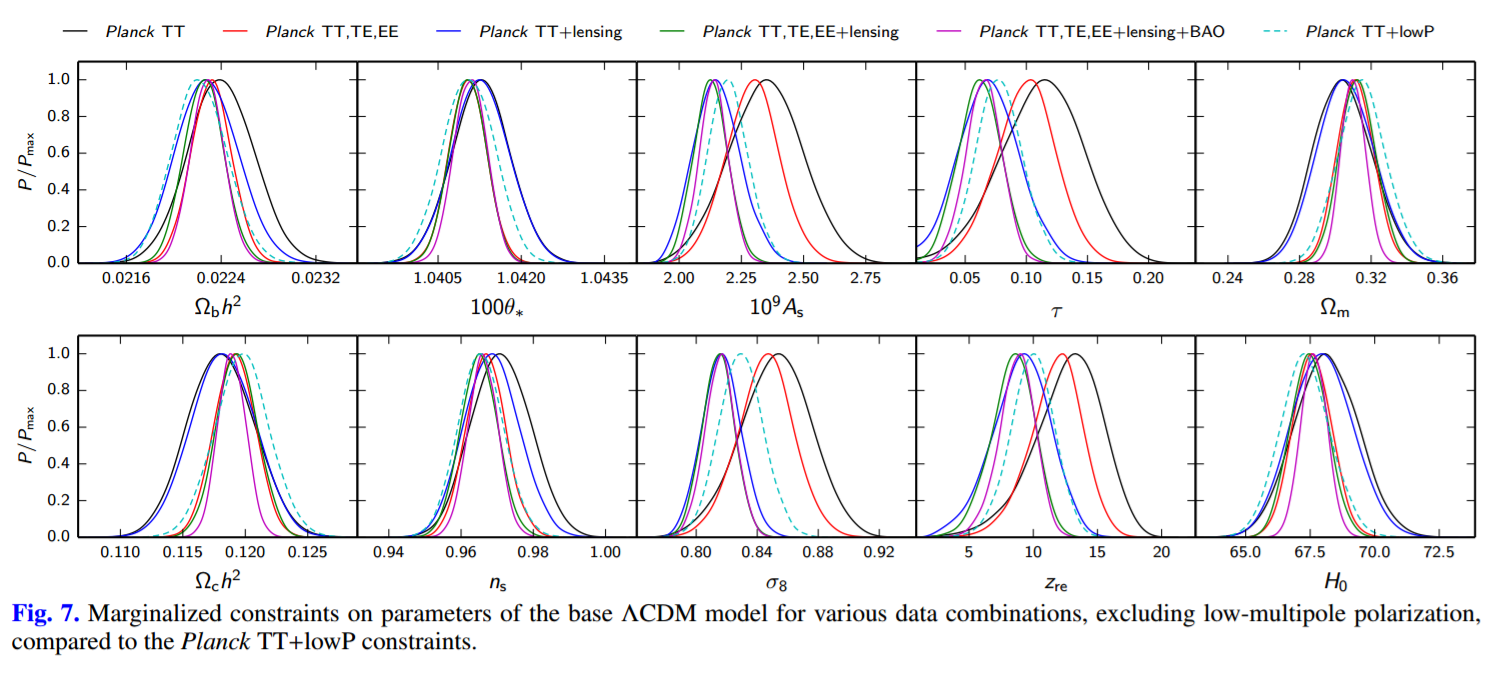
\includegraphics[width=\textwidth,angle=0.]{lambdaCDMconstraints.png}
\end{center}
\caption{Constraints on many $\Lambda$CDM parameters, including $\Omega_b$,~$\Omega_c$, and $\Omega_m$. From Ref. 1}
\end{figure}

\subsection*{2. Hinshaw et al 2013: Nine-year WMAP Observations}
\begin{itemize}
\item $\Omega_\Lambda=.7185$ to within 1.5\%
\item Fit to 6-parameter model
\end{itemize}

\newpage
\section{Growing Entropy: Comments}
The arguments for the second law of thermodynamics to hold are pretty convincing to me. In addition, Ref. 2 uses data from Ref. 1 to show that entropy will eventually reach a maximum; i.e. entropy is increasing. Ref. 3 also shows more qualitative theoretical arguments. I didn't see anything arguing that the entropy of the universe should be decreasing. This feature makes sense to me. 

\newpage
\section*{1. Growing Entropy: Evidence}
\subsection*{Simon et al 2005: Constraints on the redshift dependence of the dark energy potential}
\begin{itemize}
\item Determine shape of dark energy potential
\item From this, get Hubble evolution: $H'(a)<0$, $H''(a)>0$
\end{itemize}

\begin{figure}[h]
\begin{center}
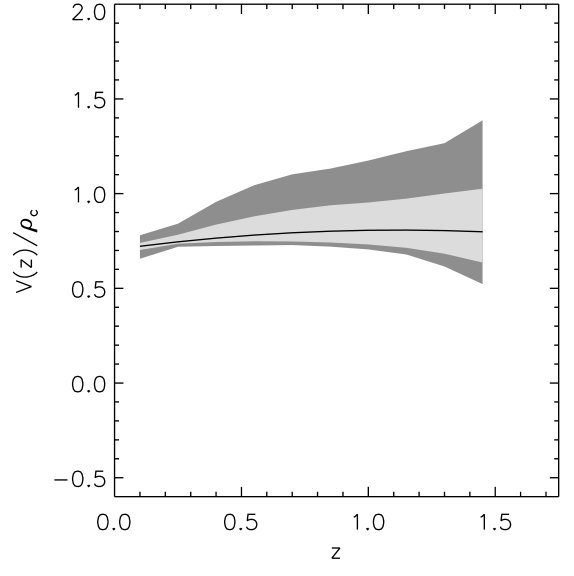
\includegraphics[width=.5\textwidth,angle=0.]{entropy1.png}
\end{center}
\caption{Determining the shape of the dark energy potential via redshift measurements.}
\end{figure}

\subsection*{2. Pavon and Radicella 2013: Does the entropy of the Universe tend to a maximum?}
\begin{itemize}
\item Entropy grows unbounded with gravity, bounded with black holes
\item From Hubble constant evolution (Ref. 1), entropy tends toward a maximum, not unbounded
\end{itemize}

\subsection*{3. Goldstein et al 2016: Is the hypothesis about a low entropy initial state...}
\begin{itemize}
\item Low entropy evolves to higher entropy (thermo law)
\item Feynman: the past was more ordered because we expect things to look the same
\end{itemize}


\newpage
\section{Non-zero Vacuum Energy: Comments}
I think it is pretty cool that the LHC is yielding some results that can be used to look at vacuum stability. Ref. 1 does this and finds that our universe is smack in the middle of the metastable region, although confidence levels do allow for a stable or (less likely) unstable vacuum. Ref. 2 uses the $\Lambda$CDM model and varies the vacuum energy equation of state, finding a good fit for values close to $w=-1$. There is still the possibility of quintessence, phantom dark energy, and so on though so I am not totally convinced. 

\newpage
\section*{Non-zero Vacuum Energy: Evidence}
\subsection*{1. Alekhin et al 2012: The top quark and Higgs boson masses and the stability of the electroweak vacuum}
\begin{itemize}
\item Use mass from two different LHC experiments of top quark and higgs boson to constrain vacuum stability like in class
\end{itemize}

\begin{figure}[h]
\begin{center}
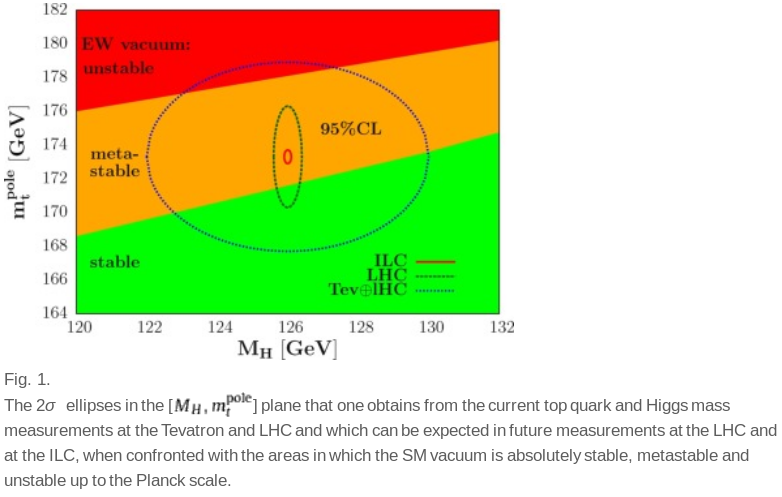
\includegraphics[width=\textwidth,angle=0.]{vacuumEnergy.png}
\end{center}
\caption{Observations from LHC (ATLAS and CMS) confine to metastable vacuum region}
\end{figure}

\subsection*{2. Planck Collaboration 2016: Planck 2015 Results}
\begin{itemize}
\item Assuming a $w=w_0+(1-a)w_a$ yields good fit to CMB data
\end{itemize}
\end{document}
